\chapter{Results}
After extensive testing of different hyperparameters, the model that produced the best accuracy was used to predict the pixel class for the data in the test dataset that was left untouched during training. 
\section{Hyperparameters}
A simple grid search was used to iterate over a list of all possible combinations for the hyperparameters, train the model for 100 epochs on each and calculate the accuracy on the test dataset. The parameters chosen are shown in Table \ref{tab.grid_search}. 
\begin{table}[htbp]
\centering 
\begin{tabular}{l|l}
                           & \textbf{Possibilities}   \\ \hline
\textbf{Number of Filters} & 2, 4, 8, 16, 32, 64      \\ 
\textbf{Learning Rate}     & 0.1, 0.01, 0.001, 0.0001 \\ 
\textbf{Batch Size}        & 16, 12, 64, 128, 256     \\ 
\end{tabular}
\caption[Hyperparameter possibilities]{Depicts all the possibilities considered for the hyperparameters chosen in this study.}
\label{tab.grid_search}
\end{table}
The following sections will show the effect of changing one of the hyperparameters while fixing the other two. The key three key characteristics to observe as mentioned in Section \ref{sec.model_training} are:
\begin{enumerate}
    \item Validation loss should be slightly higher than training loss once training is complete. Training should continue while validation loss is lower than the training loss.
    \item If training loss reduces without an increase in validation loss, training should continue
    \item Once validation loss starts to increase, training should discontinue. 
\end{enumerate}
\subsection{Adjusting the Learning Rate}
Adjusting the learning rate adjusts the length the weight vector is travelled on before the loss is calculated again for the next iteration. A smaller learning rate means a smaller adjustment to the weights between iterations. In Figure \ref{fig.lr_varied} the loss rate that shows the most optimal rate of decay is a learning rate of 0.001. After each iteration, the training loss has decrease and the validation loss has remained lower. In contrast, the loss rate for a learning rate of 0.0001 shows a lot of fluctuation in the validation loss and is not displaying a fast decay in of the loss rate. Additionally, the loss rate of 0.1 does not show much variation in the training loss, so would not be considered when continuing training. The learning rate of 0.01, while there is a great deal of fluctuation, the loss is gradually decaying over time. 
\begin{figure}[htpb]
    \centering
    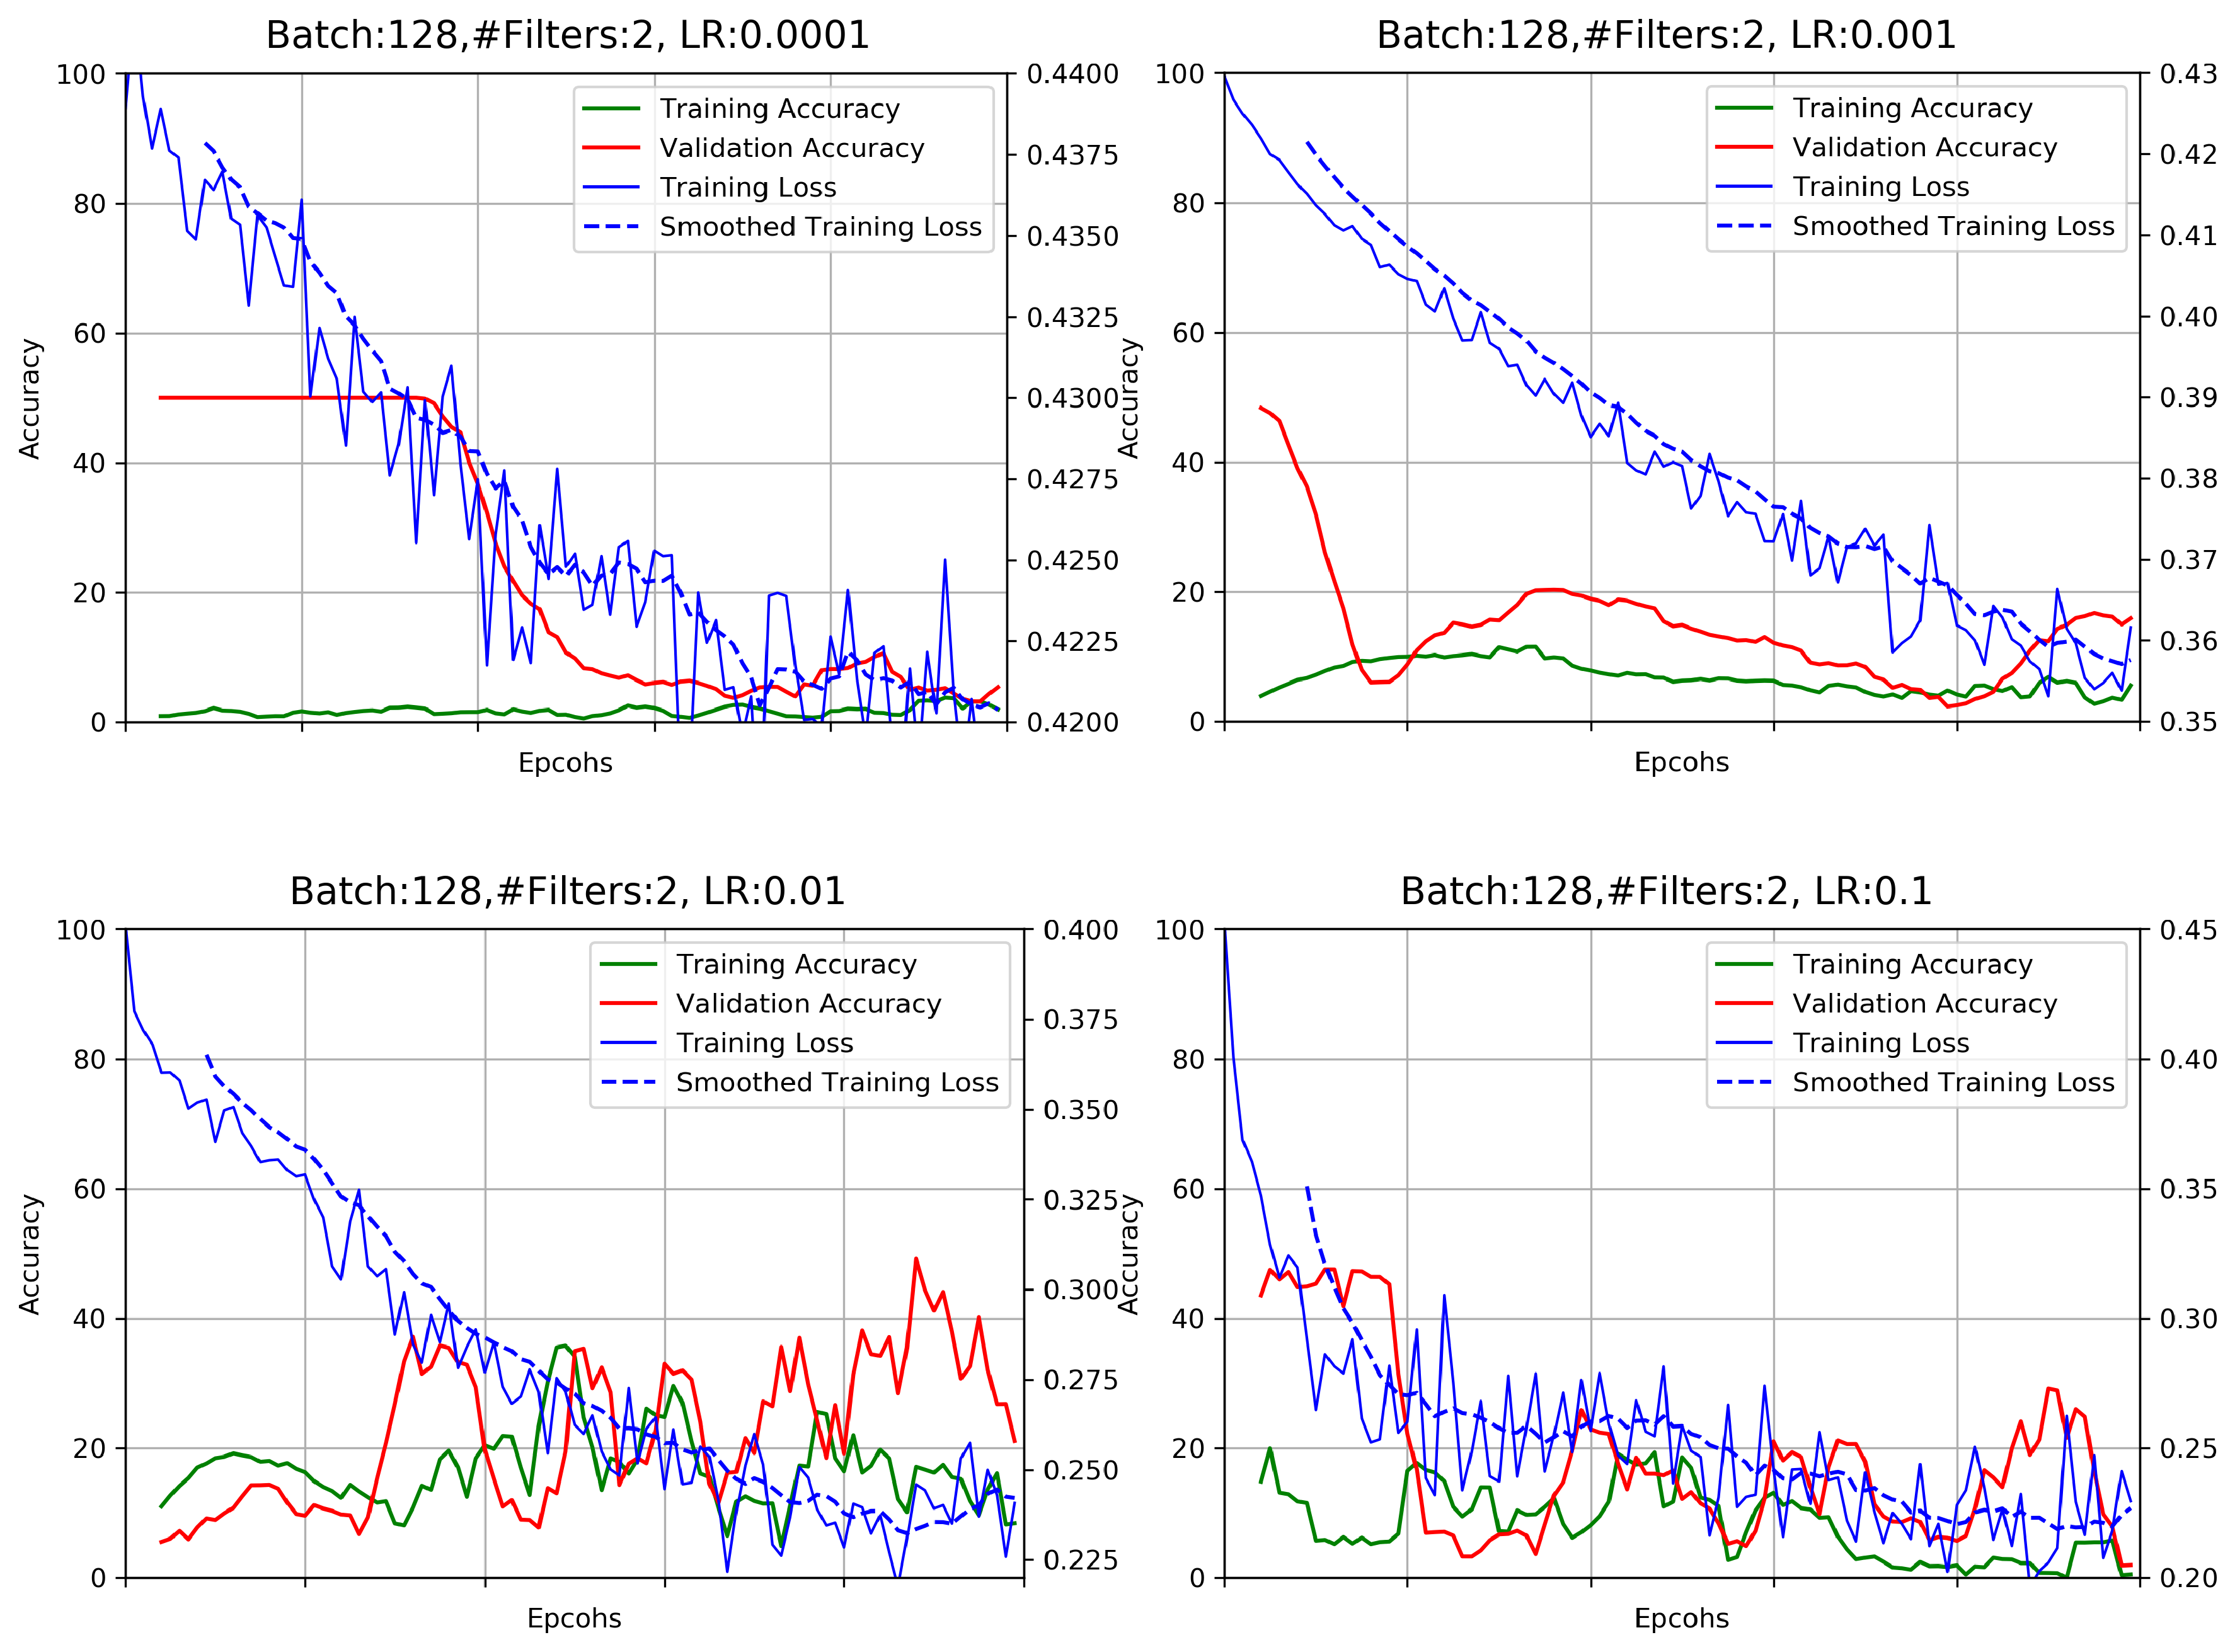
\includegraphics[width=\textwidth]{\dir/figs/lr_varied.png}
    \caption[Example of the affect of changing the learning rate]{Example of how the learning rate affects the training progression over 100 epochs.}
    \label{fig.lr_varied}
\end{figure}
\subsection{Adjusting the Batch Size}
As demonstrated in Section \ref{sec.batch_size}, changing the batch size affects the depth of the stack of training samples that input into the network on each iteration. Where the batch size is larger than the number of training samples, the batch dimension becomes the number of training samples. For the final plot, the batch size will be 108. The variability in training loss is minimal in the final plot, however, validation is greater than training loss after 100 epochs, so training cannot continue for that combination of hyperparameters. The four previous plots all demonstrate a decaying loss rate as learning progresses. However, with a batch size of 16 and 32, the validation loss has some quite large fluctuations that are greater than the training loss indicative of overfitting and making them less optimal choices as a hyperparameter. 
\begin{figure}[htpb]
    \centering
    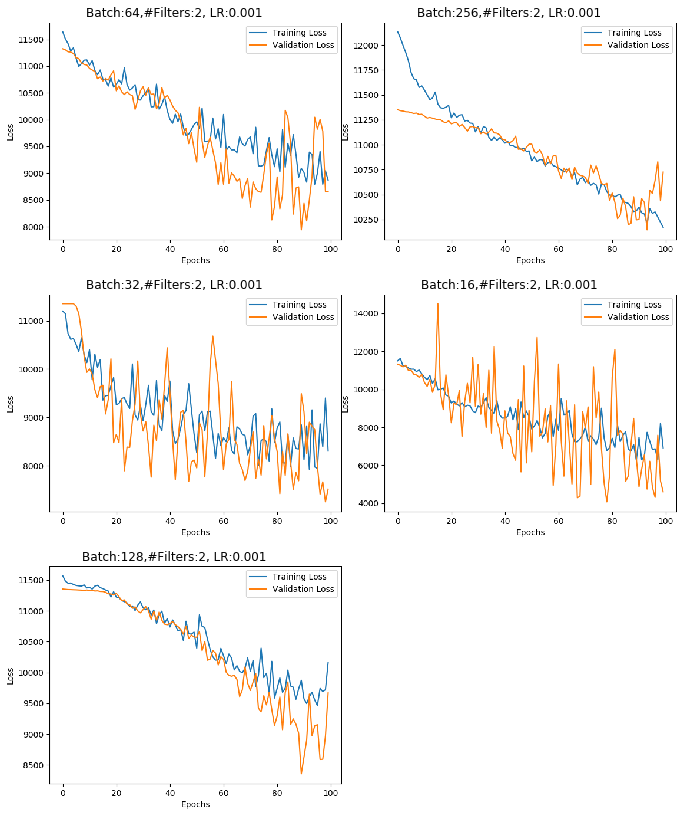
\includegraphics[width=\textwidth]{\dir/figs/batch_varied.png}
    \caption[Example of the affect of changing the batch size]{Example of how the batch size affects the training progression over 100 epochs. The number of filters and the learning rate remain fixed, while the batch size is increased by a factor of two for each of the plots.}
    \label{fig.batch_varied}
\end{figure}
\subsection{Adjusting the Number of Filters}
Adjusting the number of filters adjusts how many features are being extracted from the input image and fed into the next layer. With all of the plots, there is decaying in the loss as training progresses. In all of the figures except the first, there is large variability in validation loss with it going above the training loss on multiple occasions. This indicates that an initial filter of two is the optimal hyperparameter for this combination. 
\begin{figure}[htpb]
    \centering
    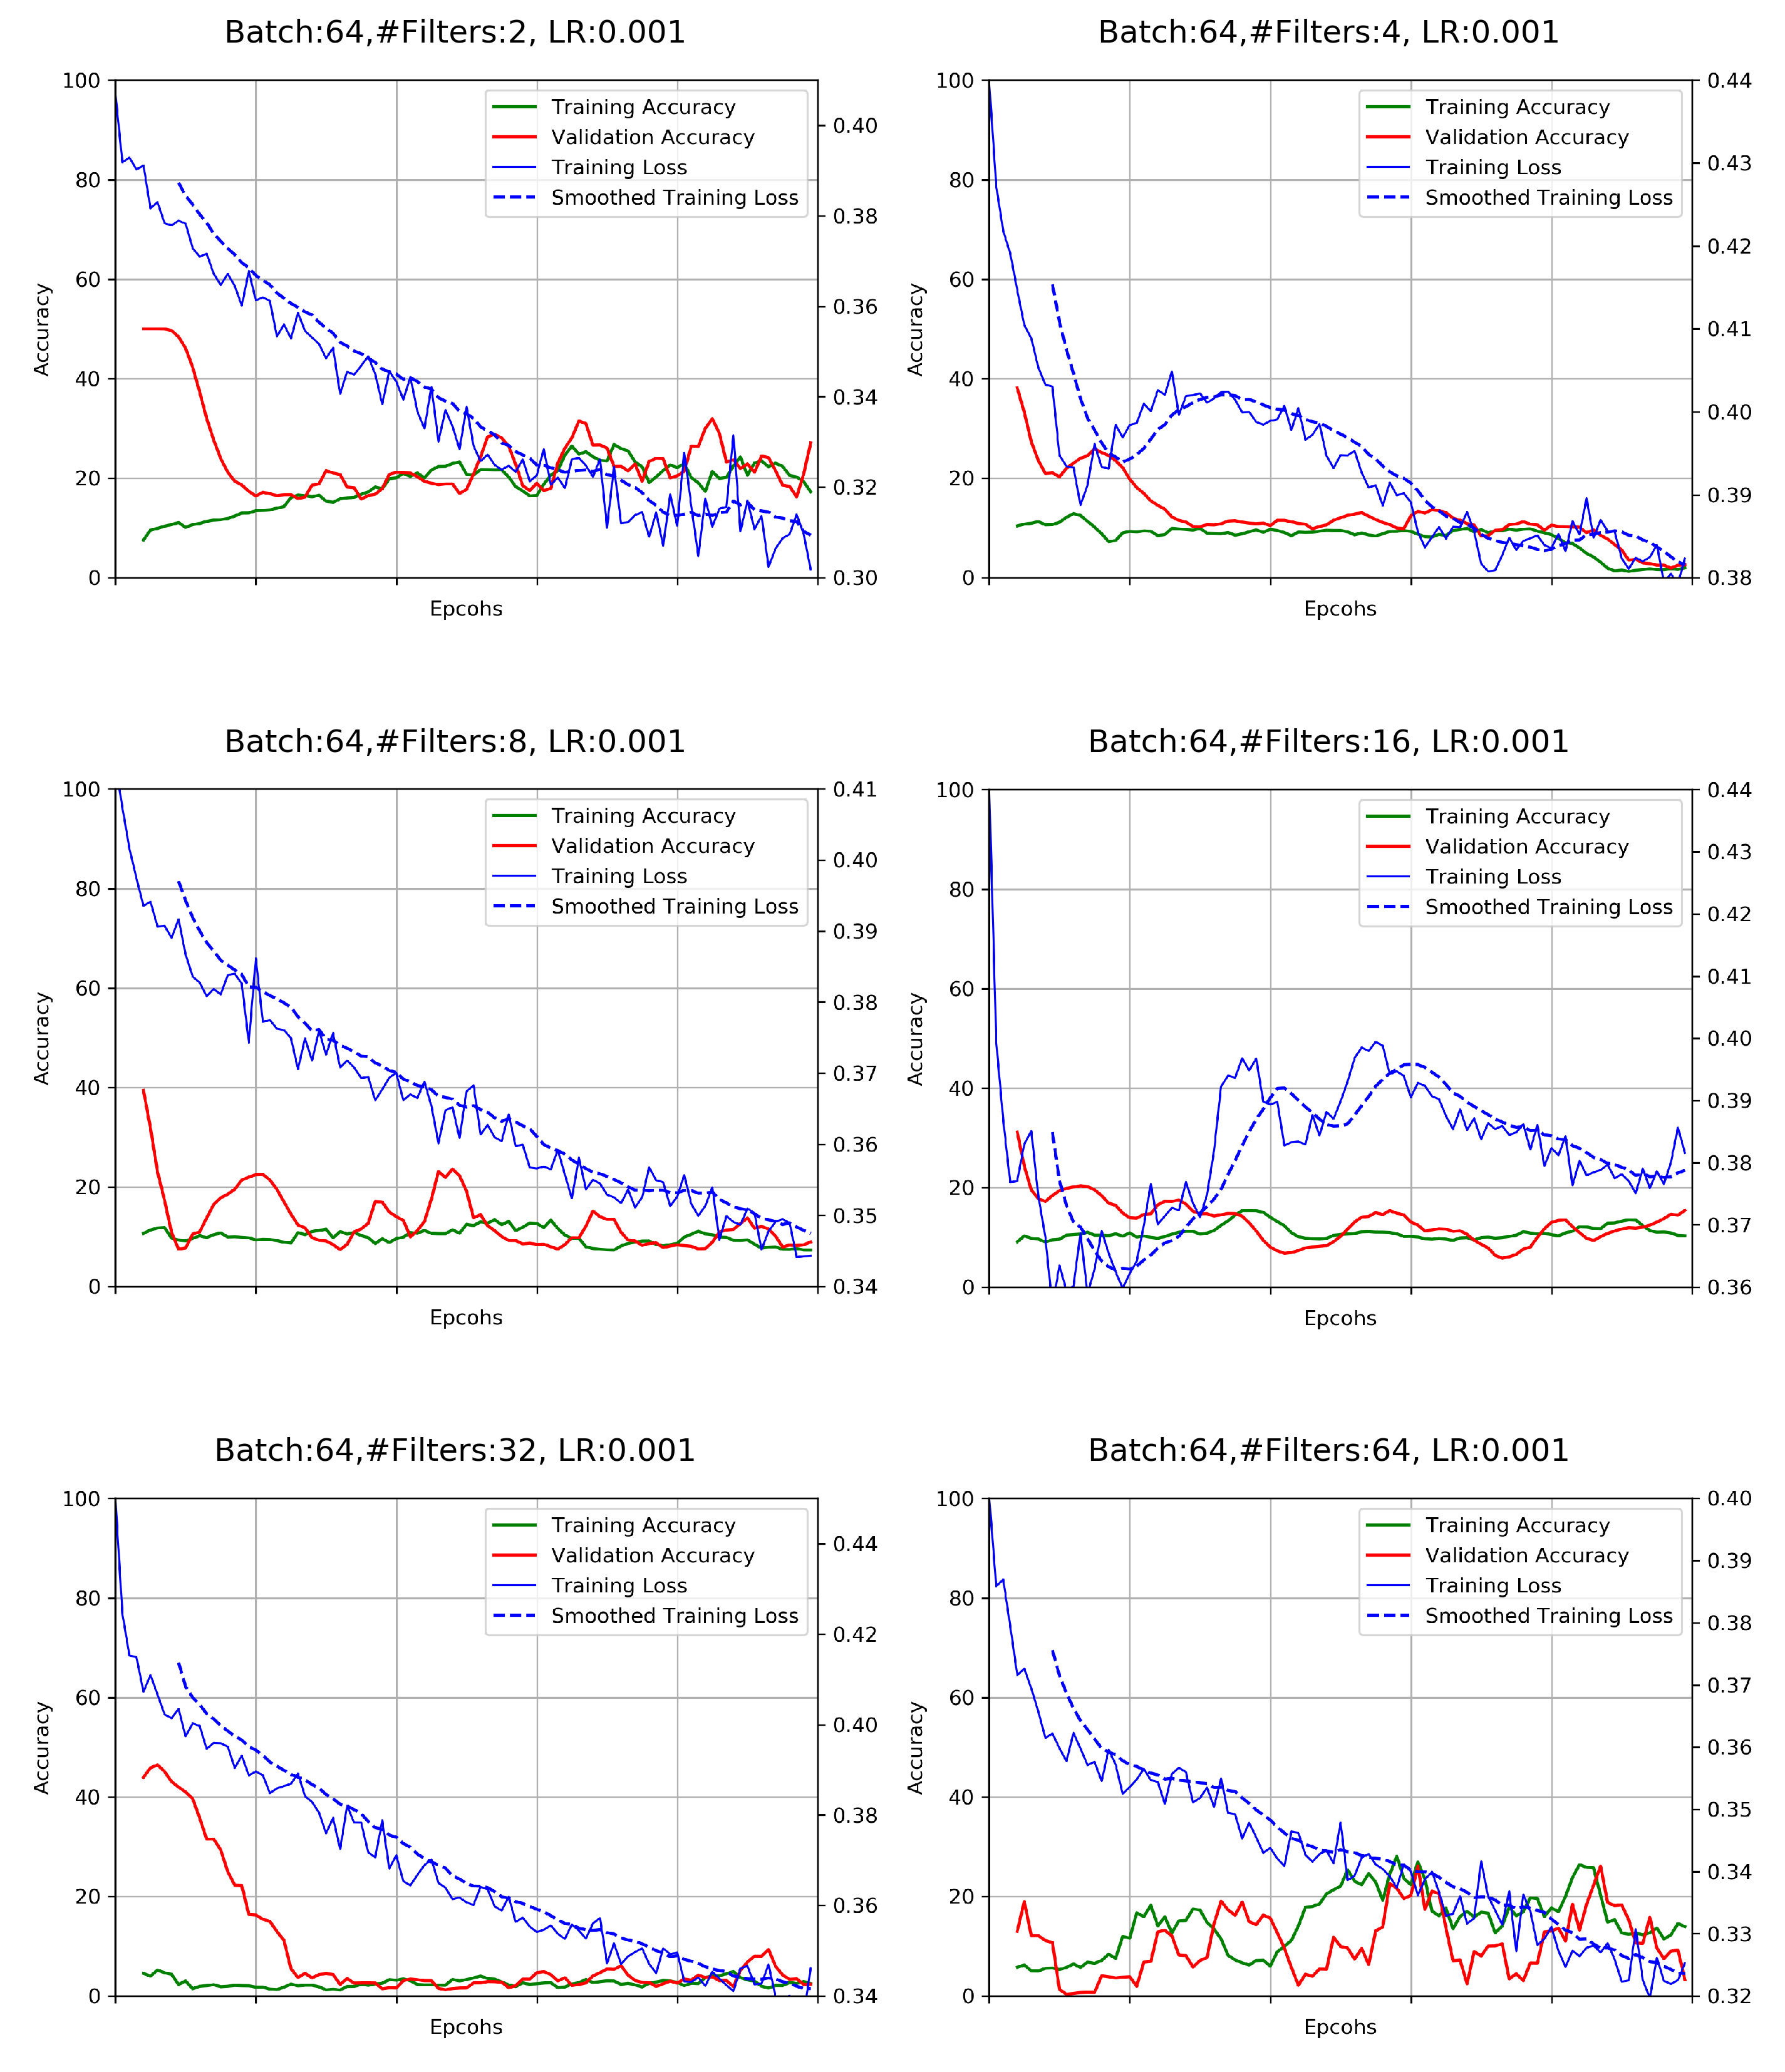
\includegraphics[width=\textwidth]{\dir/figs/net_varied.png}
    \caption[Example of the affect of changing the number of filters in each Convolution layer]{Example of how changing the number of filters affects the learning rate. The plots show the number of filters increasing from 2 to 128 by a factor of 2 each time.}
    \label{fig.net_varied}
\end{figure}
\section{Accuracy}
Throughout the training process, the network saves the state of the weights and the biases whenever the loss rate reduces. This model state can then be loaded again at a later data and training can continue. The final stage of training takes the model state that results in the lowest loss and applies it to the test data to make a prediction and evaluate the accuracy.
\par
The most accurate model is the model that will be used to make predictions on the test dataset. Table \ref{tab.hyper_param}, shows the results of training over 100 epochs for all possible combinations for the three hyperparameters. A lot of the results are not accurate, with their accuracy being below 10\%. The highest accuracy produced is 44-55\%, each of these model runs had 32 initial filters and the final two had batch sizes of 16. The most accurate model had a learning rate of 0.01 and the second most accurate had a learning rate of 0.001. 
\begin{table}[htpb]
\centering
\begin{adjustbox}{totalheight=\textheight-2\baselineskip}
\begin{tabular}{rrrrr}
\toprule
 Accuracy &   Time &  Batch Size &  Learning Rate &  Filter Size \\
\midrule
    0.000 &   5.62 &        64.0 &         0.1000 &         64.0 \\
    0.000 &   5.23 &       128.0 &         0.0100 &         16.0 \\
    0.057 &   5.33 &       128.0 &         0.1000 &         16.0 \\
    0.076 &   5.11 &        32.0 &         0.1000 &         32.0 \\
    0.243 &   5.71 &       128.0 &         0.0010 &         32.0 \\
    0.401 &   7.37 &        32.0 &         0.1000 &         16.0 \\
    0.471 &   5.06 &        64.0 &         0.1000 &         16.0 \\
    0.641 &   4.92 &        64.0 &         0.1000 &         32.0 \\
    1.398 &   6.02 &        32.0 &         0.0010 &         64.0 \\
    1.886 &   5.98 &       128.0 &         0.0100 &         64.0 \\
    2.203 &   6.03 &       128.0 &         0.1000 &         64.0 \\
    2.243 &   4.82 &       256.0 &         0.0100 &         64.0 \\
    2.258 &  10.50 &        64.0 &         0.0100 &         64.0 \\
    2.754 &   5.75 &        64.0 &         0.0010 &         64.0 \\
    3.100 &   6.32 &        64.0 &         0.0001 &         32.0 \\
    3.892 &   5.83 &       128.0 &         0.0001 &         16.0 \\
    3.904 &   5.34 &        32.0 &         0.0010 &         16.0 \\
    3.937 &   5.24 &        32.0 &         0.0100 &         64.0 \\
    4.035 &   5.06 &       128.0 &         0.0010 &         16.0 \\
    4.343 &   5.30 &        64.0 &         0.0001 &          8.0 \\
    4.548 &   5.48 &       256.0 &         0.1000 &         16.0 \\
    4.584 &   5.71 &        32.0 &         0.0100 &         16.0 \\
    5.326 &   4.85 &       256.0 &         0.1000 &         64.0 \\
    5.352 &   7.45 &       256.0 &         0.1000 &         32.0 \\
    5.995 &   5.49 &       256.0 &         0.0010 &         64.0 \\
    7.756 &   5.63 &        32.0 &         0.0001 &         64.0 \\
    7.840 &   5.92 &        16.0 &         0.1000 &         16.0 \\
    8.232 &   5.36 &        32.0 &         0.0001 &          8.0 \\
    8.282 &   4.81 &       256.0 &         0.0100 &         16.0 \\
    8.585 &   7.60 &       128.0 &         0.0100 &         32.0 \\
    8.867 &   5.29 &       256.0 &         0.0001 &         64.0 \\
    9.668 &   5.46 &        64.0 &         0.0001 &         64.0 \\
    9.826 &   5.99 &       256.0 &         0.0010 &         32.0 \\
   10.535 &   5.67 &        16.0 &         0.0001 &         32.0 \\
   10.712 &   6.65 &        32.0 &         0.0010 &         32.0 \\
   10.836 &   5.94 &        16.0 &         0.1000 &         64.0 \\
   10.853 &   5.52 &        16.0 &         0.0010 &         16.0 \\
   11.248 &   5.87 &        16.0 &         0.0100 &         64.0 \\
   12.138 &   5.22 &        32.0 &         0.1000 &         64.0 \\
   12.249 &   5.76 &       256.0 &         0.0100 &         32.0 \\
   12.302 &   5.06 &       256.0 &         0.0001 &         16.0 \\
   13.822 &   5.96 &        64.0 &         0.0100 &         16.0 \\
   14.965 &   5.97 &        16.0 &         0.1000 &         32.0 \\
   15.332 &   5.58 &        64.0 &         0.0001 &         16.0 \\
   15.789 &   5.24 &       256.0 &         0.0001 &          8.0 \\
   16.824 &   4.81 &        32.0 &         0.0001 &         16.0 \\
   17.999 &   5.52 &       128.0 &         0.0001 &          8.0 \\
   18.578 &   4.91 &       128.0 &         0.0001 &         64.0 \\
   18.845 &   4.88 &        64.0 &         0.0010 &         32.0 \\
   19.220 &   5.21 &       256.0 &         0.0010 &         16.0 \\
   19.585 &   5.35 &        16.0 &         0.0100 &         16.0 \\
   21.727 &   5.07 &       256.0 &         0.0001 &         32.0 \\
   22.014 &   5.06 &        32.0 &         0.0001 &         32.0 \\
   22.790 &   5.53 &       128.0 &         0.0001 &         32.0 \\
   23.090 &   5.22 &       128.0 &         0.0010 &         64.0 \\
   24.361 &   5.59 &        16.0 &         0.0010 &         64.0 \\
   26.538 &   4.74 &        16.0 &         0.0001 &         16.0 \\
   26.827 &   4.99 &        16.0 &         0.0001 &         64.0 \\
   37.611 &   5.16 &        64.0 &         0.0010 &         16.0 \\
   44.251 &   7.37 &       128.0 &         0.1000 &         32.0 \\
   45.031 &   5.16 &        16.0 &         0.0010 &         32.0 \\
   55.069 &   5.81 &        16.0 &         0.0100 &         32.0 \\
\bottomrule
\end{tabular}
\end{adjustbox}
\caption[Hyperparameter Search Results]{Results from hyperparameter searching to find the optimal hyperparameters with which to train the network. Accuracy is increasing with each change in model hyperparameters.}
\label{tab.hyper_param}
\end{table}
Figure \ref{fig.3d_hyperparams} shows how most hyperparameter combinations produce low accuracy. A large number of filters does not increase model accuracy. However, it is difficult to say clearly which other hyperparameter values worked well and which didn't.  
\begin{figure}[htpb]
    \centering
    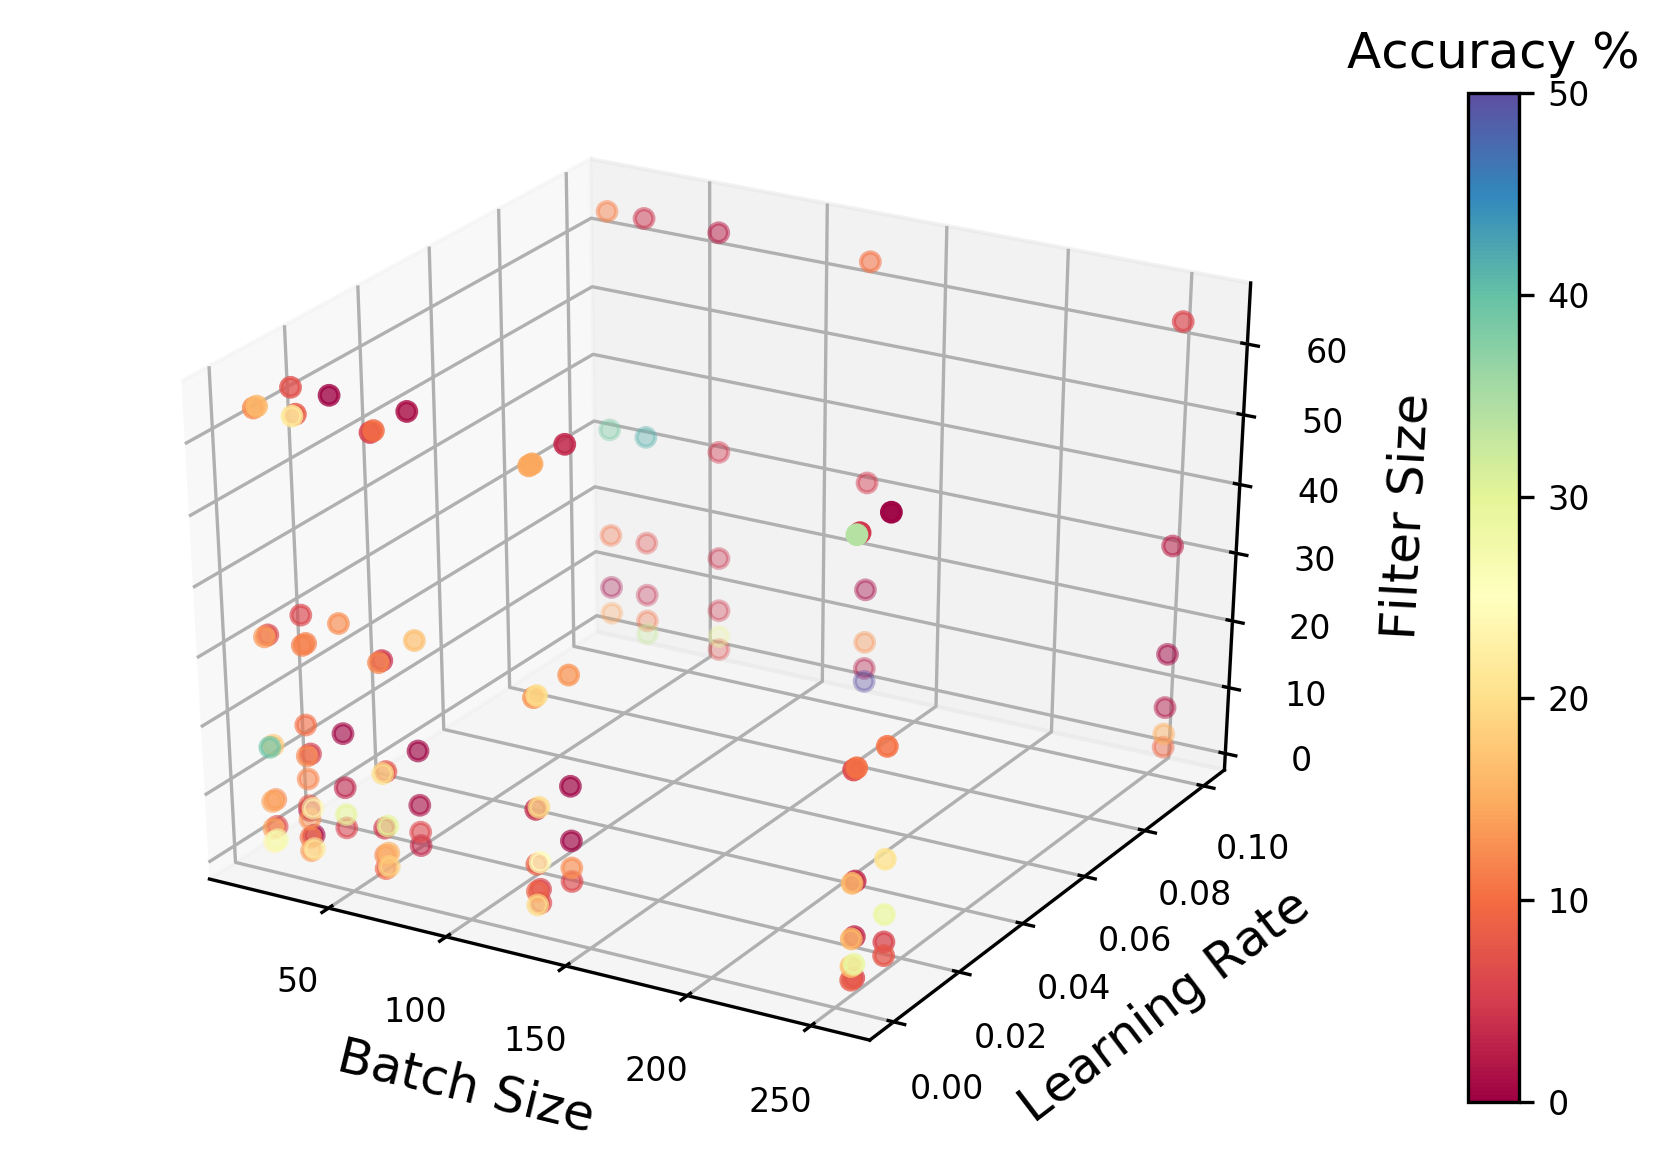
\includegraphics[width=\textwidth]{\dir/figs/3d_params.png}
    \caption[3D representation of the accuracy of different hyperparameter combinations]{A 3D representation of Table \ref{tab.hyper_param} plotting the three hyperparameter and colouring them according to their accuracy. Points that are bluer in colour represent ones that produce an accuracy approaching 50\%.  }
    \label{fig.3d_hyperparams}
\end{figure}
\section{Predictions}
To see how well the model has predicted where building are or aren't, the weights and biases of the network are fixed and all the images are sequentially passed through the network and a prediction made on a pixel by pixel basis. Figure \ref{fig.prediction} shows the result of the prediction on the same images as exampled in Figure \ref{fig.inria_dataset}. 

\begin{figure}[htpb]
    \centering
    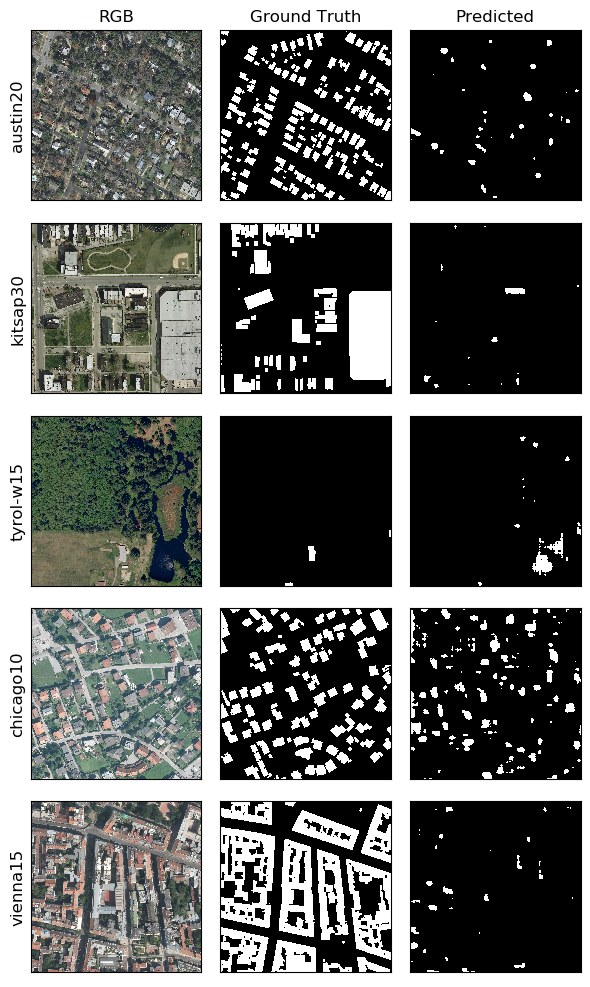
\includegraphics[height=\dimexpr \textheight - 4\baselineskip\relax]{\dir/figs/Predicted_Grid.png}
    \caption[Image Prediction using the model with the best accuracy]{Image prediction using the model trained with the hyperparameters that produce the highest accuracy. Side by side comparison of the ground truth labels and the model prediction is clearly shown.}
    \label{fig.prediction}
\end{figure}

Tile together the rasters from all of the different places, then confusion matrix each one to see how accurate the model was for each city... That is the final result